\section{3-Phase Job Model}
\label{Sec:Model}

\begin{figure}[htp]
        \centering
        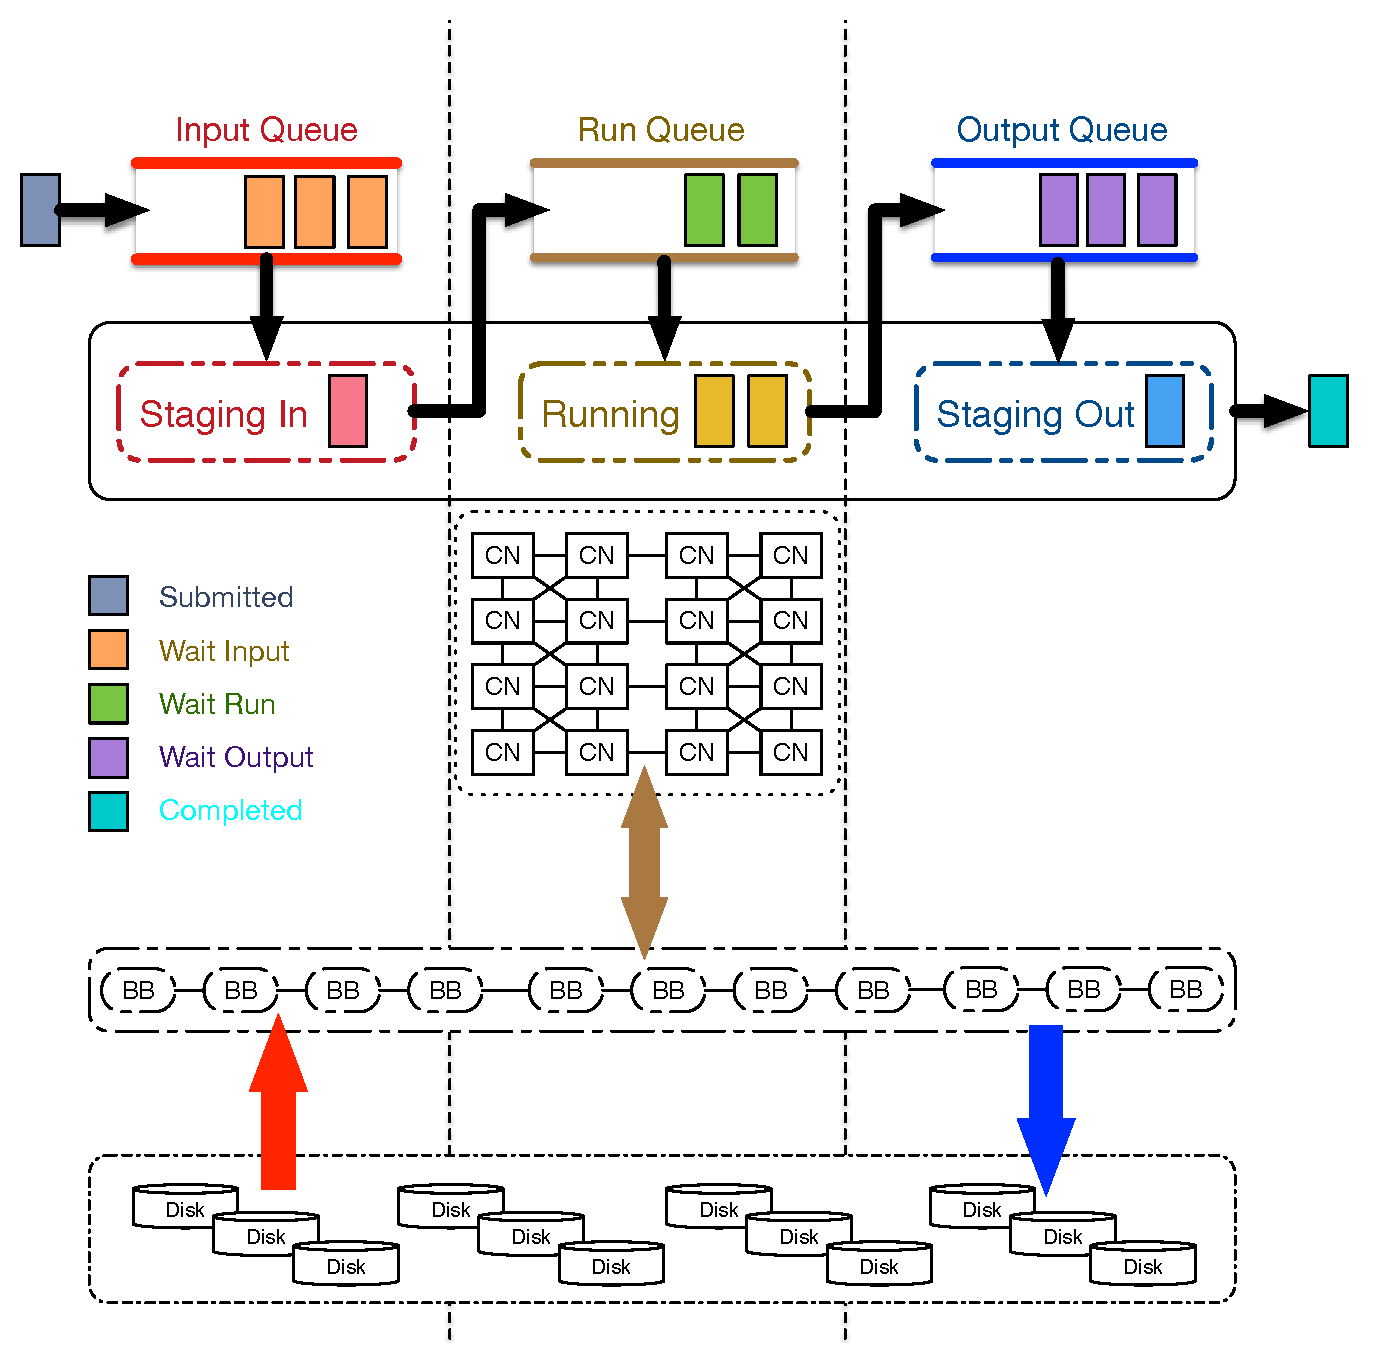
\includegraphics[width=3.6in]{CerberusBBSystem}
        \caption{The design of 3-Phase burst buffer aware scheduling. The black arrows indicate 
        the jobs changing of status; the red, peru and blue arrows in the bottom indicate the data flow in different phases. \TODO{you need to show Q\_I, Q\_R,Q\_O in the figure!!!-lan} }
        \label{Fig:CerberusQueues}
\end{figure}

The traditional batch scheduler on a system without burst buffer only considers
the job with the number of required nodes and the expected runtime for the scheduling decision making process.
The most commonly used scheduling policy is the First Come First Serve with EASY backfilling~\cite{tsafrir-tpds-2007}.
However, on burst-buffer-enabled systems,
the amount of available burst buffer capacity becomes a new scheduling constraint.
We propose Cerberus, a burst-buffer-aware batch scheduler.
Cerberus takes the advantage of the most common use cases of burst buffer:
data stage-in, checkpointing, and data drain-out.
Cerberus allocates burst buffer in each phase for one of the three use cases
by maintaining three distinct queues, as shown in Figure~\ref{Fig:CerberusQueues}.
%Before entering each phase, job must enqueue to the corresponding queue.
The input queue $Q_I$ contains all the jobs that need to pre-fetch data from the external storage to the burst buffer.
The running queue $Q_R$ holds the jobs that are waiting for the compute nodes and the burst buffer used for checkpointing.
Jobs waiting to be drained out to the external permanent storage are in the output queue $Q_O$.
The layered hierarchy in Figure~\ref{Fig:CerberusQueues} also indicates that burst buffer
can fill in the memory gap between the memory on compute nodes and the hard disk storage.


Before we give the details of our Cerberus design, 
in this section we describe our 3-Phase job model 
and the corresponding resource demand at each phase. 
We assume that upon job submission, 
a user specifies the amount of compute nodes, 
the expected job runtime, 
and the amount of burst buffer needed by his/her job. 
The batch scheduler makes scheduling decisions according to job requirements, 
with the objective to maximize job performance and system utilization.

%The batch scheduler makes scheduling decisions for 
%each job based on its demand while attempting to
%minimize the overall job response time and maximize the system throughput.
%However, jobs requiring more than one resource could result in possible deadlocks and starvation.
%In order to improve the overall resource utilization and the system responsiveness, we propose
%a fine granularity job model based on the possible use cases of burst buffer.
%In our scheduling framework, the system resources include compute nodes and burst buffer.
%The job resource demand varies in different execution phases;
%Correspondingly, the batch scheduler makes scheduling decisions in each phase.


% Users request the system to run their applications as jobs.
% We define $J = (job_1, job_2, \ldots, job_n)$ to be the set of all unfinished jobs in the system.
% To fully utilizing burst buffer, we divide jobs into 3 different phases.
% In the first phases, input data are staged in from IO nodes to burst buffer.
% We refer this phase as \textit{stage-in} phase.
% It is very easy for user to provide the amount of input data
% because they should already be available before application execution. 
% Then the job can run on the compute nodes after being scheduled;
% except reading data from burst buffer, there may be interaction between 
% computer node and burst buffer.
% These interactions are mainly due to fault tolerance reasons, like check-pointing.
% This phase is called \textit{running} phase.
% When computation is done, output data needs to be staged out to external PFS from memory,
% namely \textit{stage-out} phase.
% Burst buffer plays as an efficient IO broker for compute nodes,
% in replacing of traditional IO nodes.


%=============Xu======================
%\subsection{Three-Phase Job Model}
Applications can benefit from burst buffer in three major ways\cite{BBUseCase}.
Before execution, job pre-fetch data from the external storage to the burst buffer.
When jobs start running on the compute nodes,
they could burst the checkpoint data to the burst buffer at high speed.
Upon the job completion, 
useful output data are staged out to the burst buffer for early releasing the compute nodes.
Therefore, we divide the job lifetime into three different phases, as illustrated in Figure~\ref{Fig:CerberusQueues}. \NOTE{I prefer we keep this paragraph. Because it explains why 3-Phase make sense. 3-Phase is based on app's use case of bb.}
 
\textbf{Stage-In}: After submitting the job to the system,
         Cerberus needs to pre-fetch data, such as configuration files and input data,
         from IO nodes to the burst buffer. We define this phase as \textit{stage-in}.
         The only resource needed by the job in this phase is the burst buffer.
         Users are encouraged to specify the amount of burst buffer required in the \textit{stage-in} phase.
         The job is ready to run when the data is pre-fetched into the burst buffer.
 
\textbf{Running}: The scheduler allocates the job with the required
         number of compute nodes and the amount of burst buffer. 
         It then dispatches the job to the system for running.
         This is defined as \textit{running} phase.
         During the running phase, there could be frequent data exchange
         between the compute nodes and the burst buffer.
         These interactions, such as like check-pointing, are mainly for achieving system fault tolerance. 
 
\textbf{Stage-out}: When the job finishes computation and
         exits the \textit{running} phase, its output data need to be drained out
         to the external storage from the on-node memory. We define this as \textit{stage-out} phase.
         The job can release its compute nodes when the output data are staged out
         into the burst buffer at high speed. The burst buffer serves as an efficient
         IO broker for the compute nodes and drains the output data to the external storage.

%While burst buffer has been utilized during all three phases,
%compute nodes are only required during the \textit{running} phase. 


%\subsection{Three-Phase Resource Demand Model}
% Users typically provide their resource demand for their jobs.
% This is the most important information scheduler could get from the users.
% Therefore, each job is associated with a demand vector in the form of $(c, rt)$
% where $c$ is the number of needed compute node in running phase,
% $rt$ is the requested runtime user can provide to help scheduler make decisions.
% To be burst buffer aware, demand vector should be augmented
% with fields defining user's request for burst buffer capacity.
% We consider two possible ways to do so.
% Corresponding to the typical usage cases of burst buffer,
% user may provide a \textit{burst buffer triple} in the form of $(bb\_in, bb\_run, bb\_out)$,
% where $bb\_in$ is the volume of burst buffer user predicted for staging in data files,
% $bb\_run$ is the volume of burst buffer user preferred for checkpointing during running,
% $bb\_out$ is the volume of burst buffer needed to hold the resulting output data.
% A job that providing demand vector augmented with
% burst buffer triple is called a \textit{3-phase modeled job}.
% Alternatively, a lazy user may just use the $\max\{bb\_in, bb\_run, bb\_out\}$ at every stage.
% %We do not make any assumption about $bb\_run$ and $bb\_out$
% %because it is nontrivial to predict them, both for system scheduler and application owner.
% We refer this augmentation as
% \textit{1-phase modeled jobs} thereafter.

%=========XY===============
Jobs are submitted to the system with the specified resource demand.
Each job is associated with a demand vector in the form of $(c, ert)$,
where $c$ is the number of needed compute nodes in the running phase,
$ert$ is the expected runtime.
In a burst-buffer-enabled system, the demand vector should be augmented
with fields defining user's requests on the burst buffer capacity.
We consider two possible ways that users provide the burst buffer demand.
For the users with accurate speculation about their job's burst buffer demand in each phase,
they may provide a \textit{burst buffer triple} in the form of $(bb\_in, bb\_run, bb\_out)$,
where $bb\_in$ is the volume of burst buffer for staging in data files,
$bb\_run$ is for checkpointing during the execution, and
$bb\_out$ is for staging out the output data.
% A job that providing demand vector augmented with
% burst buffer triple is called a \textit{3-phase modeled job}.
We will show the benefits of providing the job burst buffer demand in the form of \textit{burst buffer triple} in the next section.
Alternatively, a user may just use the $\max\{bb\_in, bb\_run, bb\_out\}$
as the job's burst buffer demand in the whole lifetime.
% We refer this augmentation as
% \textit{1-phase modeled jobs} thereafter.

% The tightly coupling between processing cores and memory makes 3-phase model
% more complicated than it appears in terms of resource releasing.
% For a job at the stage-in phase, compute nodes is not allocated to it yet
% but that will not effect staging in data.
% When scheduler allocate compute nodes (coupled with memory) to a job,
% these nodes are exclusively used by this job.
% The first thing to do in running phase is fetching in data from burst buffer to memory,
% which is not available until compute nodes is allocated to job.
% We refer this sub-phase as \textit{fectch-in} phase.
% $bb\_in$ will be hold by job until \textit{fetch-in} phase finished.
% Even if the computation is done when job exit \textit{running phase},
% compute nodes cannot be released until job enters \textit{stage-out} phase 
% \textbf{and} output data are drained out to burst buffer from memory,
% referred as \textit{drain-out} phase.
% However, $bb\_run$ can be immediately reclaimed at the end of \textit{running phase}.
% Once \textit{drain-out} phase is done,
% compute nodes become available for jobs waiting to be run
% because staging output data out to IO node is the business of burst buffer nodes,
% sometimes with the help from traditional IO nodes.
% Burst buffer nodes used for caching output data can thus be put back for reuse
% when \textit{stage-out} phase, as well as the entire lifetime of job, concludes.



%The resource releasing for the 3-phase modeled jobs is nontrivial. 
%For a job at \textit{stage-in} phase, compute nodes is not allocated to it yet. 
%The job can stage in data from external storage to burst buffer without the involvement of compute nodes.
%When scheduler allocates compute nodes to the job, the job enters the \textit{running} phase 
%and starts to read the pre-fetched data from burst buffer into the main memory, 
%$bb\_in$ will be released after all the data are moved into main memory. 
%When the job finishes computation and exits \textit{running} phase, 
%$bb\_run$ are released while compute nodes are still hold by the job. 
%The compute nodes will be released after all the output data are moved into $bb\_out$ from main memory.
%The job at \textit{stage-out} phase only holds $bb\_out$ burst buffer. 
%Once all the output data are drained out to the external storage,  
%$bb\_out$ is released.


\begin{table}[ht] 
        \renewcommand{\arraystretch}{1.3}
        \caption{Summary of Symbols}
        \label{Tab:Symbols}
        \centering
        \begin{tabular}{l|l}
                \hline
                $CN$ & number of total compute nodes \\
                $BB$ & amount of total burst buffer nodes \\
                $CN_{available}$ & number of available compute nodes \\
                $BB_{available}$ & amount of available burst buffer nodes \\
                $c_i$ & compute node demand of $job_i$ \\
                $bb\_in_i$ & burst buffer demand of $job_i$ at \textit{stage-in} phase \\
                $bb\_run_i$ & burst buffer demand of $job_i$ at \textit{running} phase \\
                $bb\_out_i$ & burst buffer demand of $job_i$ at \textit{stage-out} phase \\
                $rt_i$ & running time of $job_i$ recorded in the log trace \\
                $ert_i$ & estimated or expected running time of $job_i$ \\
                $Q_I, Q_R, Q_O$ & queues for \textit{stage-in, running, stage-out} phases \\
                $J_{Q_I}, J_{Q_R}, J_{Q_O}$ & set of jobs in corresponding queues \\
                $\mathcal{J}_{Q_I}, \mathcal{J}_{Q_R}, \mathcal{J}_{Q_O}$ & selected jobs from the corresponding queues\\
                $p_i$ & profit of $job_i \in J_{Q_R}$ \\
                $dp(\cdot)$ & memo used in dynamic programming \\
                \hline
        \end{tabular}
\end{table}

